\documentclass{beamer}
\usepackage[utf8x]{inputenc}
%\usepackage{default}
\usepackage{verbatim}


\newcommand{\projectName}{ACHTBITS}
\newcommand{\projectAbbreviation}{Awesome
CHaradriiformes Toegepast BIrd Tracking System}


\title{\projectName}
\subtitle{\projectAbbreviation}
\author{Jesse Eisses, Sosha Happel, Maarten Inja and Maarten de Waard}
\institute{UvA}
\usetheme{Berkeley}
\newcommand{\slide}[2]
{
\begin{frame}
\frametitle{#1} 

#2

\end{frame}
}



\begin{document}
\begin{frame}
\titlepage
\end{frame}



\section{Introductie}
\slide{Het Project}
{
UvA-bits verzamelt GPS en accelerometerdata van vogels

Onze focus: Kleine mantelmeeuw
\vspace{0.5cm}

Onderzoeksdoelen:
\begin{itemize}
	\item Automatische segmentatie van datapunten
	\item Classificatie van gedrag boven de Noordzee
	\begin{itemize}
		\item 'Directional flight'
		\item 'Searching'
		\begin{itemize}
			\item 'Foraging'
			\item 'Trawler'
		\end{itemize}
		\item 'Floating'
		\begin{itemize}
			\item Sleeping'
			\item 'Digesting'
		\end{itemize}

	\end{itemize}
\end{itemize} 
}

\slide{Problemen}
{
Meeste problemen zaten in de data zelf
\begin{itemize}
	\item Veel onbruikbare data
	\item Weinig features
	\item Geen geannoteerde data
	\item Annoteren is erg lastig
\end{itemize} 
}

\slide{Plan}
{
Zo veel mogelijk automatisch
\begin{itemize}
	\item Data opsplitsen in bruikbare sessies
	\item Sessies automatisch segmenteren in clusters
	\item Nieuwe features maken voor clusters
	\item Annoteren versimpelen
	\item Clusters classificeren met nieuwe features
\end{itemize} 
}

\section{Preprocessing}
\slide{Data opsplitsen in sessies}
{
\begin{itemize}
    \item Alles boven de noordzee weggooien
    \item Data mag niet `NULL' zijn.
    \item Minimaal 1 uur
    \item Gewenste resolutie
    \item Geen te grote gaten tussen datapunten
\end{itemize}
}

\slide{Clusters vinden (oude methode)}
{
     Alleen kijken naar snelheid.\\
     Pieken vinden:
 \begin{itemize}
    \item Kijk of de waarde van het snelheidsverschil groter is dan een
    threshold
    \item Loop door deze waardes, en markeer een cluster voordat de waarde omhoog
    gaat, of nadat deze omlaag gaat.
 \end{itemize}
    Pieken clusteren:
    \begin{itemize}
 \item The time elapsed between two peaks
 \item The difference between the current time elapsed between peaks, and the
 current cluster's average
 \item The difference between the time elapsed between the first peak of the
 cluster, and the average of the rest of the cluster.
 \end{itemize}

}


\slide{Clusters vinden (nieuwe methode)}
{
    Gebruik van histogrammen.
\begin{enumerate}
    \item Interpoleren
    \item Trainingshistogrammen maken
    \item Loop over data
    \begin{itemize}
        \item Histogram maken van huidige data
        \item Histogrammen vergelijken
    \end{itemize}
\end{enumerate}

Formule voor vergelijken histogrammen:\\
\hspace{.5cm} $Diff =  \sum \left| currentHists - exampleHists
\right|$\\
\hspace{.5cm} $percentage = 100 - \frac{Diff}{2 \sum Histogram} \times 100$
}

\begin{frame}
\frametitle{Voorbeeld}
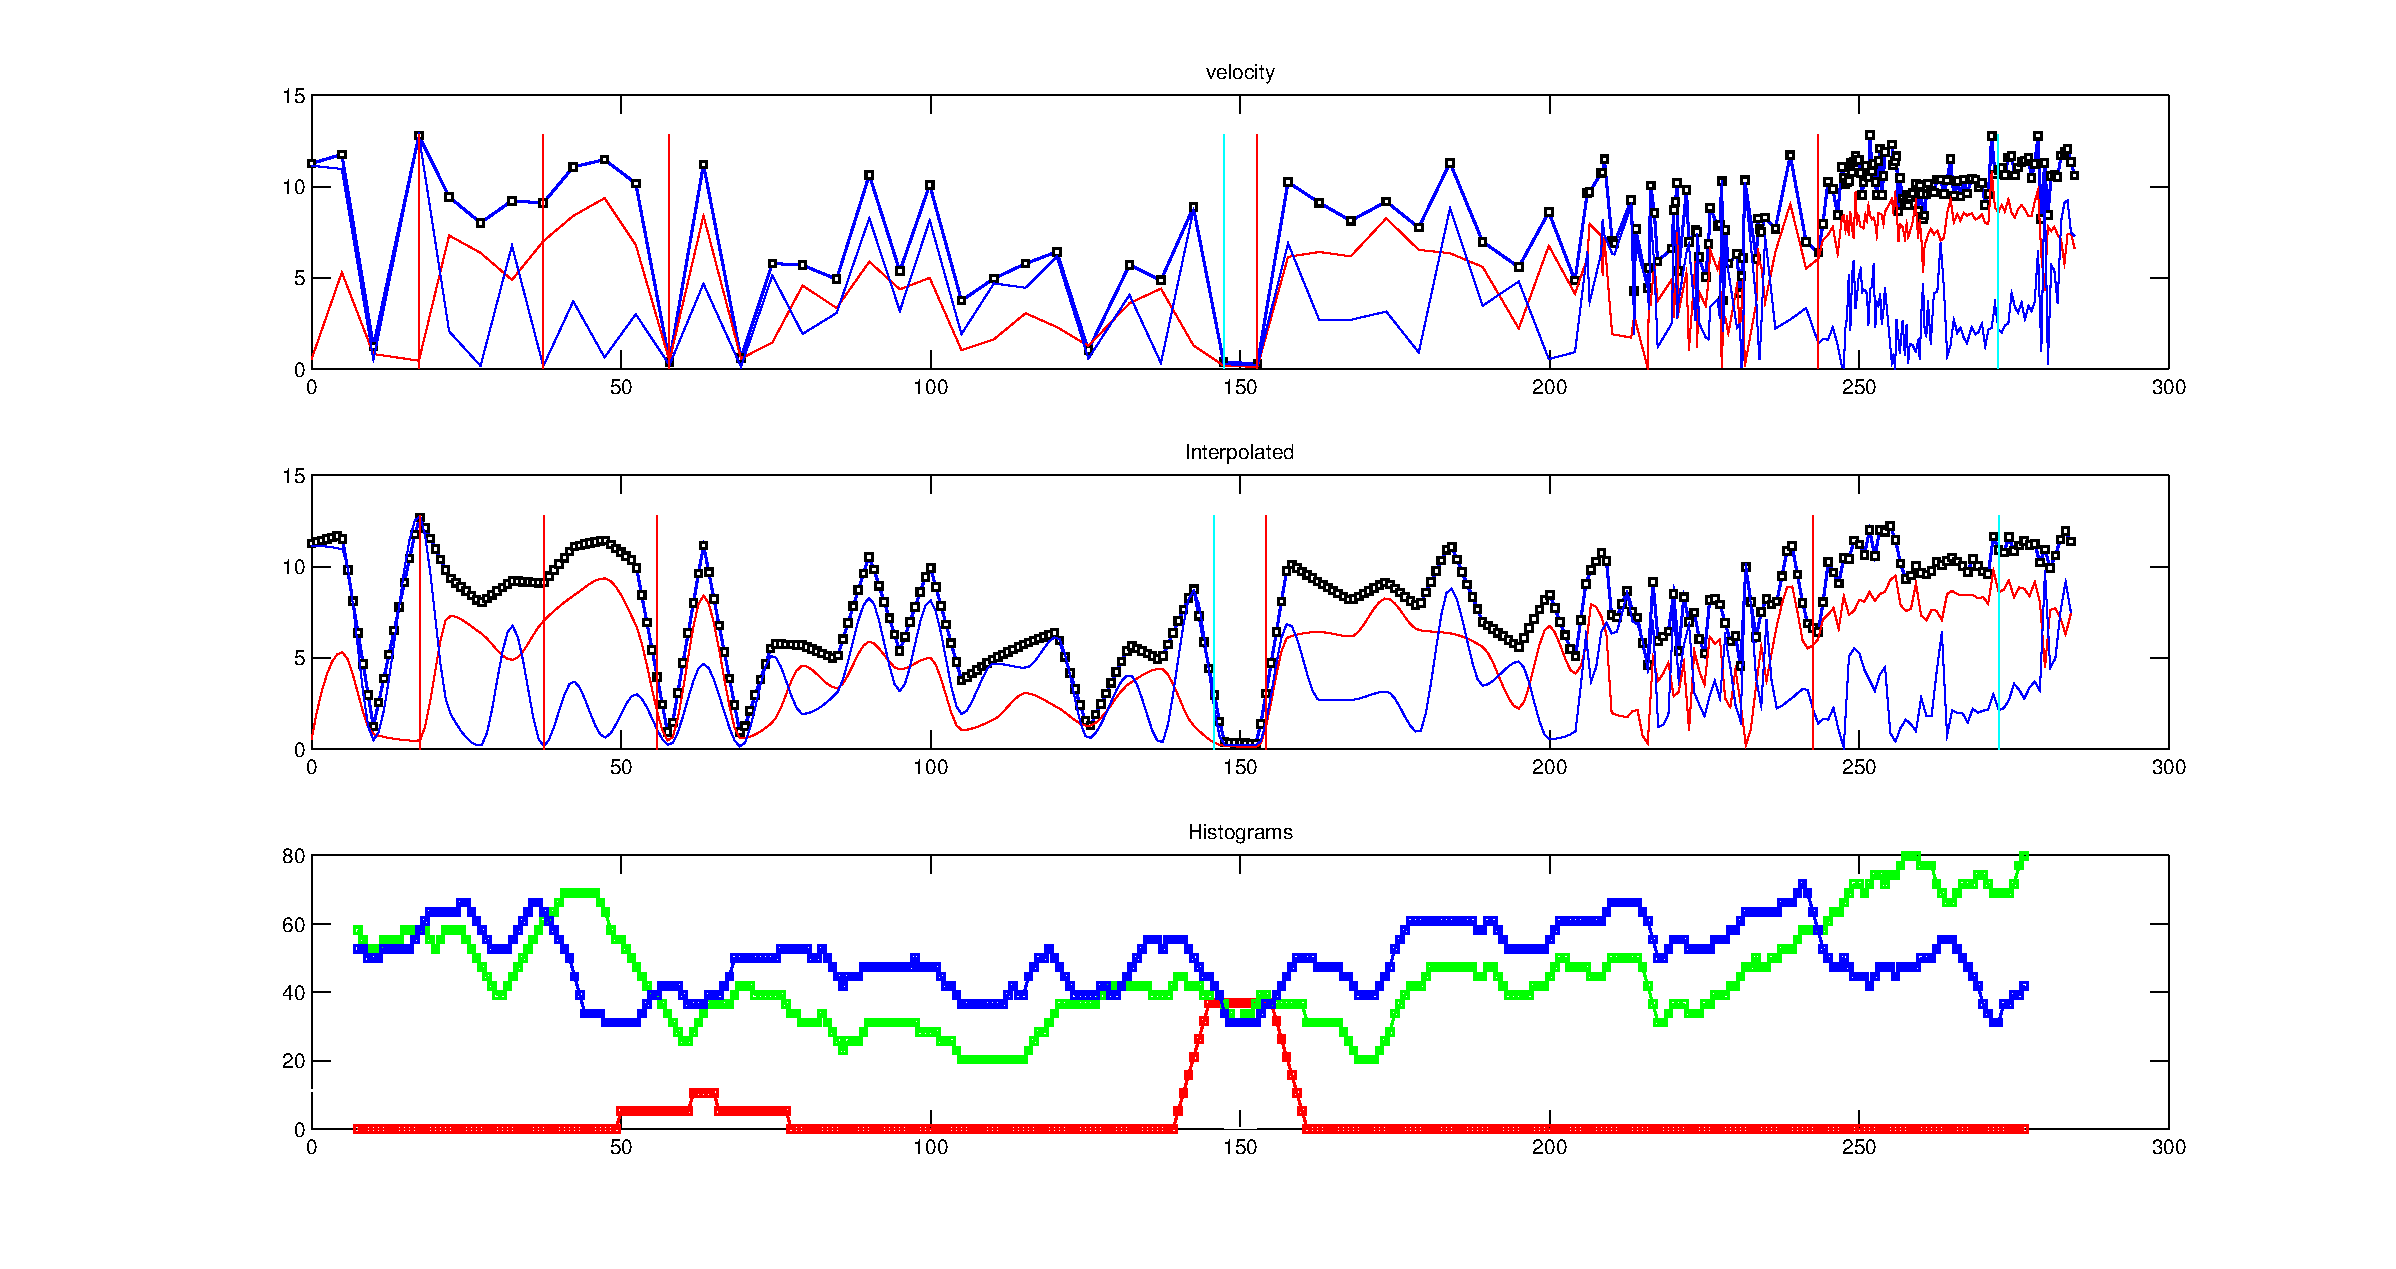
\includegraphics[width=\textwidth]{clustering.pdf}
\end{frame}


\section{Resultaten}
\slide{Annotatietool}
{
	Tool gemaakt in Matlab die de data verwerkt en het annoteren makkelijker maakt
}

\slide{Classification}
{
Cluster classificatie met WEKA:
\begin{itemize}
    \item We gebruikte 12 features
    \item Meer dan 1600 geannoteerde \emph{goede} clusters
    \item 3 klassen: 'Directional flight', 'Searching', 'Floating'
    \item Precisie van 82\% (met logistische regressie)
    \item Veel ruimte voor verbetering\ldots
\end{itemize}
\vspace{1cm}
\begin{itemize}
\item Goede features: Gemiddelde snelheid, Afgelegde afstand
\item Slechte features: Hoogte verschil, Richtings verandering
\end{itemize}
}

\section{Conclusie}

\slide{Conclusie}
{
\begin{itemize}
	\item Automatische segmentatie lijkt goed gelukt met histogrammen, alleen is lastig te meten
	\item Classificeren op 'directional flight', 'searching' en 'floating' werkt goed
	\item Onderscheid maken tussen 'sleeping' en 'digesting' is nog niet goed gelukt
	\item Annoteren is een stuk makkelijker geworden
\end{itemize} 
}

\slide{Future work}
{
\begin{itemize}
	\item Automatische segmentatie verbeteren
	\item Annotatie tool uitbereiden met suggesties
	\item Features uitbereiden
	\item Classificeren met annotatie van experts
\end{itemize} 
}
\end{document}
